\chapter{Performance Analysis}
\label{chapter:analysis}

We will now look at the performance profile of various network
configurations.

As we are running these benchmarks on the Mininet simulator, there
are natural limits on how realistic the results will be.  However, we should
be able to get good \textit{relative} results.   Therefore we will first
need to establish a baseline to which we will compare the
Paxos\index{Paxos!performance} implementation.

Instructions on how to run these tests are given in
\ref{chapter:appendix.benchmark} \vpageref{chapter:appendix.benchmark}.

\section{Baseline --- ICMP Ping on L2 Learning Switch}
\label{chapter:baseline.benchmark}

All our controllers use the L2 learning switch\index{learning switch}\index{switch!L2 learning}
from chapter \ref{chapter:l2.learning.switch} to forward packets on the
network.
%
We can therefore use a setup with only these L2 learning switches
as a basis for our performance tests.
%
We will use the topology in figure
\ref{figure:baseline.topology} and send \ac{ICMP} ping\index{ping} packets from one end of
the network to the other.
%
The reason for removing the fall-back link between $S_1$ and $S_3$ in figure
\ref{figure:graph.three.switches} is to prevent the packets from taking
different paths on the network.

\begin{figure}[ht]
  \centering
  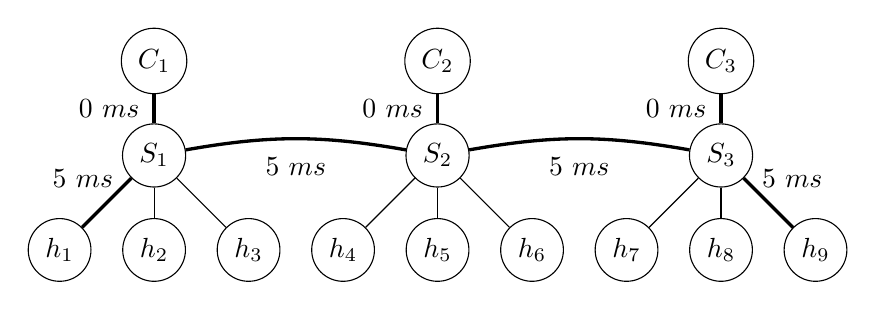
\begin{tikzpicture}[
    every node/.style={draw, circle},
    x=0.6cm,
    y=0.6cm]

    % Switches
    \foreach \n in {1,2,3} {
      \pgfmathsetmacro\x{(\n-2)*6}

      % Switch
      \node (S\n) at (\x ,  0) {$S_\n$};

      % Controller
      \node (C\n) at (\x ,  2) {$C_\n$};
      \draw (S\n) -- (C\n);

      % Hosts
      \foreach \h in {1,2,3} {
        \pgfmathsetmacro\pos{(\h - 2)*2}
        \pgfmathtruncatemacro\num{((\n - 1)*3) + int(\h)}

        % Host node
        \node (h\num) at (\x + \pos, -2) {$h_{\num}$};
        \draw (S\n) -- (h\num);
      }
    }

    % Switch links
    \draw (S1) to[out=10,in=170]
               node[below=-0.2cm, draw=none] {$5~ms$} (S2);

    \draw (S2) to[out=10,in=170]
               node[below=-0.2cm, draw=none] {$5~ms$} (S3);

    % Mark traversal path
    \draw [very thick] (h1) -- node[above left=-0.1cm,draw=none] {$5~ms$} (S1);
    \draw [very thick] (S1) -- node[left,draw=none] {$0~ms$} (C1);
    \draw [very thick] (S1) to[out=10,in=170] (S2);

    \draw [very thick] (S2) -- node[left,draw=none] {$0~ms$} (C2);
    \draw [very thick] (S2) to[out=10,in=170] (S3);

    \draw [very thick] (S3) -- node[left,draw=none] {$0~ms$} (C3);
    \draw [very thick] (S3) -- node[above right=-0.1cm,draw=none] {$5~ms$} (h9);
  \end{tikzpicture}
  \caption{Baseline topology with three switches $S$ and their controllers
           $C$. Node $h_1$ will send ICMP ping packets to $h_9$.
           The packets will go through four links with a configured
           latency of $5~ms$ and back again.
           We assume that link-latencies between switches and
           controllers are practically near zero.}
  \label{figure:baseline.topology}
\end{figure}

The first ICMP ping request from $h_1$ will cause all switches to
rebroadcast the packet to all their ports.  When the ping reaches $h_9$,
it will send back a reply, causing all controllers to learn both
the source and destination ports for $h_1$ and $h_9$.
At this point in time, the controllers can install flow table entries to
automatically forward packets to the known ports.

We will run the test twice: Once using flow tables for forwarding, and once
without.  When not using flows, the controller will issue a \textit{forward
packet to port} to the switch for each packet.

\subsection{Linear Relationship of Expected \acs{RTT}}

Before we present the results, let's look at what we should expect from the
configuration above \cite{DBLP:conf/cnsm/PhemiusB13}.

Using the link-latency\index{link-latency} $L$ and node
processing\index{processing-delay} time $P$, and a constant $K$ for
background noise, we would expect the \acf{RTT}\index{round-trip time}
between $h_1$ and $h_9$ to be

\begin{gather}
  RTT_{h_1, h_9} = 2\left( \sum_{n=1}^4 L_n + \sum_{n=1}^3 P_{S_n} +
      \sum_{n=1}^3 P_{C_n} \right) + P_{h_1} + P_{h_9} + K
  \label{equation:baseline.rtt}
\end{gather}

We can simplify by assuming that the controller processing time $P_C$ will
be negligible when complete flow entries have been installed, as the
switches will then handle the forwarding themselves.  During this initial
ramp-up, $L_{C,S} \to 0$ as $P_C \to 0$.  We will also ignore the few
cycles spent on ICMP-processing, setting $P_{h_1}$ and $P_{h_9}$ to zero.
As we will not attempt to measure $K$, we will simply set it to zero as
well.

Using the link latencies $2\sum_n^4 L_n = 2\cdot4\cdot\ms{5} = \ms{40}$
and our simplifications above,
\begin{align}
  RTT_{h_1,h_9} &= \ms{40} + 2\sum_n^3 P_{S_n} + 2\sum_n^3 P_{C_n} \\
                &= \ms{40} + 6P_S + 6P_C
  \label{equation:expected.baseline.rtt}
\end{align}

\subsection{Results}

Results for the two tests are shown in table
\ref{table:rtt.baseline.summary} and figure
\ref{figure:baseline.combined.summary.plot}.

\begin{figure}
  \centering
  \includegraphics[width=\textwidth]{data/pings-combined-summary.pdf}
  \caption{\acs{RTT}s for baseline test.  Medians are shown in red and the
    mean values in dashed blue.
    These plots do not show the large \acs{RTT}s during ramp-up.
    The first row shows \acs{RTT} for switches using flow table entries for
    packet forwarding.  The second row are measurements when using the
    controller to forward packets.  The last row plots both of them.
    Note that the histograms have a long tail. We only plot up to $\ms{100}$.}
  \label{figure:baseline.combined.summary.plot}
\end{figure}

\input{data/pings-combined-summary.tex}

There is a noticeable ramp-up as port numbers are learned and packets are
rebroadcast.  After some time, the \acs{RTT}s seem to get more steady.
Because of this short period of high \acs{RTT}s---compared to the total number of
samples---we will use the \textit{median} as a more realistic value for the
RTT. We also see that the RTT is consistently above the theoretical minimum
of $\ms{40}$.

Using the median RTT\index{round-trip time} for the first run (with flows)
in equation \ref{equation:expected.baseline.rtt}, we can estimate $P_S$.

\input{data/pings-results.tex}

The value for $P_S$ in the first run should be very near the value for the
second run, because the switch still needs to forward packets.  The only
difference between the runs is that, in the first, it must perform a flow
table match, and in the second, it must forward the packet to the
controller.  We will therefore use the value of $P_S$ in the first run to
estimate $P_C$ in the second run.

\input{data/pings-noflows-results.tex}

Again, we would like to reiterate that we are running these tests on a
\textit{simulator}.  That is why the results match so well with the expected
\acs{RTT}.  We also made a \textit{Q-Q plot}\index{Q-Q plot} (see
fig.~\ref{figure:pings.qqplot}) to see if the samples were normally
distributed, and---indeed---they match perfectly (except for the ramp-up
phase).

\begin{figure}[H]
  \centering
  \includegraphics[width=\textwidth]{data/pings-qqplot.pdf}
  \caption{Q-Q plot for ICMP ping RTT (ms).}
  \label{figure:pings.qqplot}
\end{figure}

This is most likely because the underlying simulator uses some
\acf{PRNG}\footnote{Or other, implicit means.} to produce simulated latencies.  But our
benchmarks will still be useful to us.  Using the same topology and link
latencies, we can easily see what kind of implementation techniques that
will make the system more responsive.


\section{RTT for Paxos-on-controller}

Here, we present our results of handling Paxos entirely on the controller.
For reference, we use the topology given in figure
\vref{figure:paxos.on.switches}, using events from tables
\vref{table:complete.match.leader} and \vref{table:complete.match.slave}.

From the host $c_1$, we sent UDP messages containing the client's host name,
a sequence number and the current date and time to hosts $h_5$, $h_8$
and $h_9$, measuring the \acf{RTT}.  These messages were sent at the same
time from $c_1$, and the client waited for replies from all three hosts
before sending another one.  Only a hundred messages were sent, but should
give an indication of performance.

Paxos-ordering was performed for each UDP packet going from $c_1$ to the
hosts $h_5$, $h_8$ and $h_9$, but no ordering were done for the replies,
which were forwarded using the L2 Learning Switch from section
\vref{chapter:l2.learning.switch}, running on the
OpenFlow controller.

The results are given in table \ref{table:paxos.ctrl.results} and plotted in
figure \ref{figure:paxos.ctrl.results}.

\begin{table}
  \centering
  \begin{tabular}{|l|l|l|l|l|}
    \hline
      \textbf{} &
      \textbf{$h_5$ RTT} &
      \textbf{$h_8$ RTT} &
      \textbf{$h_9$ RTT} &
      \textbf{Combined}
      \\

    \hline \textbf{Minimum} & 54.21 & 95.35 & 54.21 & 54.21 \\
    \hline \textbf{Median} & 135.06 & 139.16 & 97.44 & 117.90\\
    \hline \textbf{Mean} & 131.00 & 143.85 & 104.69 & 126.50 \\
    \hline \textbf{Max.} & 277.13 & 227.80 & 212.01 & 227.80 \\
    \hline
  \end{tabular}
  \caption{Results of 100 round-trip times from $c_1$ in ms.}
  \label{table:paxos.ctrl.results}
\end{table}

While the maximum values were in the same range, there were some variations in
the median values.  Surprisingly, $h_9$, which has the longest path from $c_1$,
has the lowest mean and median round-trip time.

The host $h_9$ also showed consistently more stable RTTs.
We have not done any further analysis on the load of various links, but
there could for instance be timing issues between the Paxos messages, in the
way the system has been set up, that consistently lead to better performance
for $c_1 \leftrightarrow h_9$.  However, this is mere speculation, and a
more detailed analysis would be called for.

The interesting part is comparing the combined values against the results in
table  \vref{table:rtt.baseline.summary}.  It shows that the medians between
these results and the flowless one in table \ref{table:rtt.baseline.summary}
differs by a factor of $1.4$, or about $\ms{34}$.  As these complete packets
are sent up from the switch to the controller, down again and then onwards,
    this is not too bad.

\begin{figure}
  \centering
  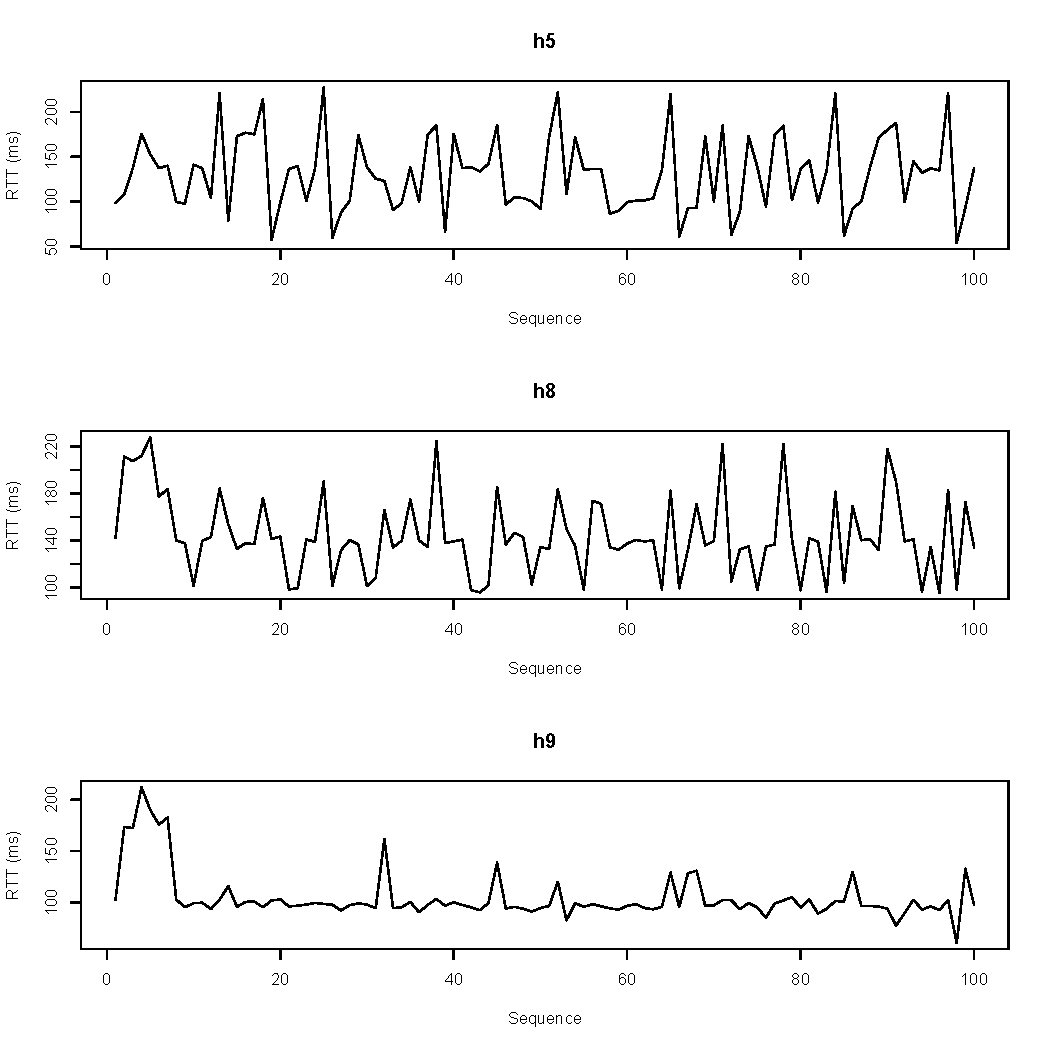
\includegraphics[width=\textwidth]{rtt-hosts.pdf}
  \caption{Results of 100 round-trip times from $c_1$.}
  \label{figure:paxos.ctrl.results}
\end{figure}

